\documentclass[11pt,a4paper,titlepage,draft]{article}
\usepackage[utf8]{inputenc}
\usepackage[greek]{babel}
\usepackage{amsmath}
\usepackage{amsfonts}
\usepackage{amssymb}
\usepackage{commath}
\usepackage{xcolor}
\usepackage{hyperref}
\usepackage[skins,theorems]{tcolorbox}
\usepackage{titlesec}
\usepackage{circuitikz}
\usepackage{pgfplots}

\usetikzlibrary{arrows.meta}

\usepackage[left=2cm,right=2cm,top=2cm,bottom=2cm]{geometry}

\makeatletter
%\newcommand{\attnboxed}[1]{\textcolor{red}{\fbox{\normalcolor\m@th$\displaystyle#1$}}}
\makeatother
\tcbset{highlight math style={enhanced,colframe=red,colback=white,%
  arc=0pt,boxrule=1pt,shrink tight,boxsep=1.5mm,extrude by=0.5mm}}
\newcommand{\attnboxed}[1]{\tcbhighmath[colback=red!5!white,drop fuzzy shadow,arc=0mm]{#1}}
\titleformat{\section}{\bf\Large}{Κεφάλαιο \thesection}{1em}{}
\newtcolorbox{attnbox}[1]{colback=red!5!white,%
  colframe=red!75!black,fonttitle=\bfseries,title=#1}
\newtcolorbox{infobox}[1]{colback=blue!5!white,%
  colframe=blue!75!black,fonttitle=\bfseries,title=#1}
  
\pgfplotsset{compat=1.12}

\title{Σημειώσεις Διαφορικές Εξισώσεις}
\date{2016, Εαρινό εξάμηνο}
\author{Καναβούρας Κωνσταντίνος \\ \textlatin{\url{http://users.auth.gr/konkanant}}}


\newtcbtheorem[number within=section]{theorem}{Θεώρημα}%
{colback=green!5,colframe=green!35!black,colbacktitle=green!35!black,fonttitle=\bfseries,enhanced,attach boxed title to top left={yshift=-2mm,xshift=-2mm}}{th}
\newtcbtheorem[number within=section]{defn}{Ορισμός}%
{colback=green!5,colframe=green!35!black,colbacktitle=green!35!black,fonttitle=\bfseries,enhanced,attach boxed title to top left={yshift=-2mm,xshift=-2mm}}{def}

\begin{document}

\maketitle

%\tableofcontents

\newpage

\part{Κεχαγιάς: Ολοκληρωτικοί μετασχηματισμοί}
\textlatin{(Fourier, Laplace)}
Τετάρτη 17:00-18:30

\section{Κεφάλαιο 7: Εισαγωγή στην ανάλυση του \text{Fourier}}
\begin{circuitikz} \draw
(0,0) to[american voltage source=$V$] (0,4)
      to[R=$R$] (4,4) 
      to[C=$C$] (4,0) -- (0,0);
\end{circuitikz}

H συμπεριφορά του κυκλώματος μπορεί να περιγραφεί με μια διαφορική εξίσωση.

\(Q(t)\): Το φορτίο του πυκνωτή σε χρονική στιγμή \(t\)

\begin{align*}
v_1 &= R\cdot i(t) = \frac{\dif Q}{\dif t}\\
v_2 &= \frac{Q(t)}{C} \\
&\boxed{v_1 + v_2 = V(t) \implies \frac{\dif Q}{\dif t} + \frac{Q(t)}{RC} = \frac{1}{R}V(t), \quad \text{με αρχική συνθήκη }Q(0)=0}
\end{align*}

Θα προσπαθήσω να λύσω την εξίσωση για τρεις περιπτώσεις:

\pgfplotsset{width=6.5cm}
\paragraph{}
\begin{tikzpicture}
  \begin{axis}[ 
    xlabel=$t$,
    ylabel={$V(t)$},
    axis lines=middle,
    xtick=\empty,
	ytick=\empty,
	title={$V(t)=V_0$}
  ] 
    \addplot[blue,thick,domain=0:5] {5}; 
  \end{axis}
\end{tikzpicture}
\hskip 10pt
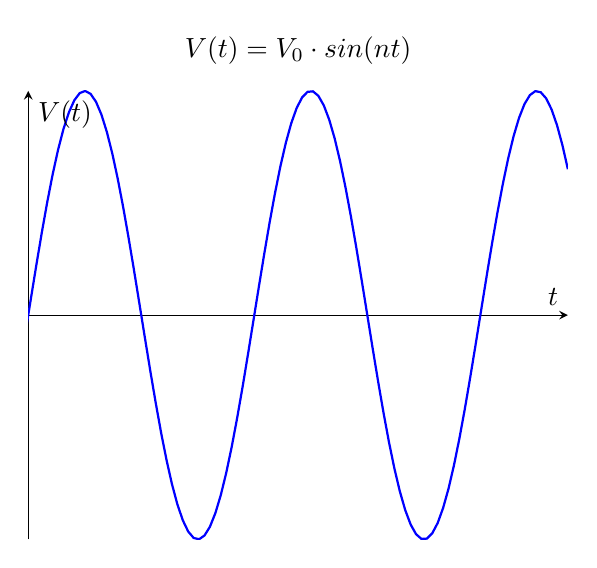
\begin{tikzpicture}
  \begin{axis}[ 
    xlabel=$t$,
    ylabel={$V(t)$},
    axis lines=middle,
    xtick=\empty,
	ytick=\empty,
	xmin=0,
	title={$V(t)=V_0\cdot sin(nt)$}
  ] 
    \addplot[blue,thick,samples=200] {5*sin(deg(3*x))}; 
  \end{axis}
\end{tikzpicture}
\hskip 10pt
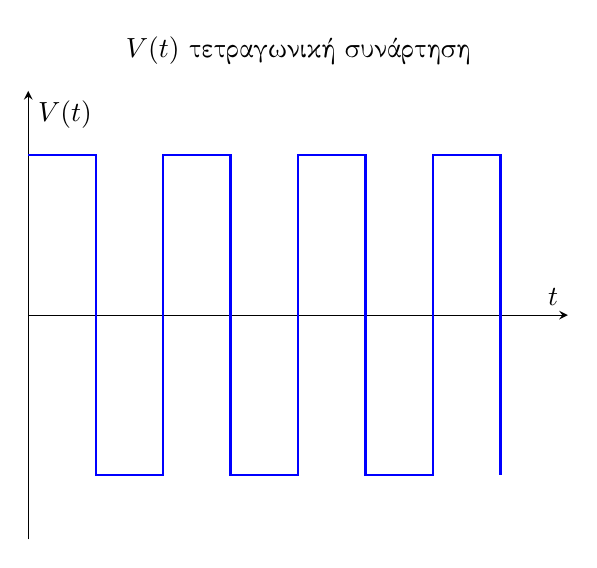
\begin{tikzpicture}
  \begin{axis}[ 
    xlabel=$t$,
    ylabel={$V(t)$},
    axis lines=middle,
    xtick=\empty,
	ytick=\empty,
	xmin=0,
	xmax=8,
	ymin=-1.4,
	ymax=1.4,
	title={$V(t)\text{ τετραγωνική συνάρτηση}$}
  ] 
    \addplot+[blue,thick,mark=none,const plot]
coordinates
{(0,1) (1,-1) (2,1) (3,-1) (4,1) (5,-1) (6,1) (7,-1)};
  \end{axis}
\end{tikzpicture}

\subsubsection{\(V(t) = V_0\)}
\[
\frac{\dif x}{\dif t}+ax=b
\]
Θα εξετάσω τη γενική λύση \(x_0(t)\) της ομογενούς ΔΕ, και \\
θα ψάξω μία ειδική λύση της μη ομογενούς ΔΕ.

Ομογενής: \(b=0 \implies \frac{\dif x}{\dif t} = -ax \implies x(t)=ce^{-at}.\)\\\(x(0)=0\implies c=0 \implies x_0(t)=0\).

Μη ομογενής: \(\frac{\dif x}{\dif t}+ax=b\).
\[
x(t)=k \implies \frac{\dif x}{\dif t}+ak=b \implies k =\frac{b}{a} \implies x(t)=k=\frac{b}{a}
\]

\begin{theorem*}{}
%\paragraph{Θ.}
Η γενική λύση της μη ομογενούς είναι:
\[x(t) = x_h(t)+x_i(t) \]
\end{theorem*}

Άρα \[
\begin{cases}
x(t) = ce^{-at} - \frac{b}{a} \\
x(0) = 0
\end{cases}
\implies 0=x(0)=c+\frac{b}{a}
\implies x(t) =\frac{b}{a}-\frac{b}{a}e^{-at} \text{ ή και }
 x(t) =\frac{b}{a}(1-e^{-at})
 \]

\begin{tikzpicture}
  \begin{axis}[ 
    xlabel=$t$,
    ylabel={$x(t)$},
    axis lines=left,
    xtick=\empty,
	ytick=\empty
  ] 
    \addplot[blue,thick,domain=0:5] {1-e^(-x)}; 
  \end{axis}
\end{tikzpicture}

 
\[
a=\frac{1}{RC}, \quad b= \frac{V_0}{R}
\]

\subsubsection{\(V(t)=V_0 \sin(nt)\)}
\[
\frac{\dif x}{\dif t} + ax = b\sin (nt)
\]

Είναι \(x_h(t) = ce^{-at}\).

Υποθέτω \(x(t) = c_2 \sin (nt) + c_3 \cos (nt) \). Τότε \( \frac{\dif x}{\dif t} = nc_2 \cos (nt) - nc_3 \sin (nt) \):

\[ \frac{\dif x}{\dif t} +ax =
\left( ac_2 - nc_3
\right)
\sin (nt) +
\left( ac_3 + nc_2
\right) \cos (nt)
= b \sin (nt) \implies
\]

\[
\implies
\begin{cases}
ac_2-nc_3&=b \\
nc_2+ac_3&=0 
\end{cases}
\implies \cdots \implies
\begin{cases}
c_2 &= \frac{ab}{a^2+n^2} \\
c_3 &= -\frac{bn}{a^2+n^2} 
\end{cases}
\]

Θυμάμαι ότι \(x(t) = x_h(t)+x_i(t) = c_1e^{-at} + \frac{ab}{a^2+n^2} \sin (nt) -  \frac{bn}{a^2+n^2} \cos (nt)\) και από το \(x(0)=0\) βρίσκω \(c_1 = \frac{bn}{a^2+n^2}\).

Άρα:
\[
x(t) = \frac{bn}{a^2+n^2} + \frac{ab}{a^2+n^2} \sin (nt) -  \frac{bn}{a^2+n^2} \cos (nt)
\]

Για το \(RC\) κύκλωμα, \(a=\frac{1}{RC} \leftarrow \) χρονική σταθερά κυκλώματος, \(b=\frac{V_0}{R}\), άρα:
\[
Q(t) = \frac{V_0C^2Rn}{C^2R^2n^2+1}e^{-\frac{t}{RC}} + \frac{CV_0\sin (nt) - C^2RnV_0 \cos (nt)}{C^2R^2n^2+1}
\]

\begin{attnbox}{}
\begin{align*}
p \cos (\omega t) + q \sin (\omega t) = \\
\sqrt{p^2+q^2} \left( \frac{p}{\sqrt{p^2+q^2}} \cos \omega t+ \frac{q}{\sqrt{p^2+q^2}} \sin \omega t \right) = \\
\sqrt{p^2+q^2} \left ( \sin \phi \cos \omega + \cos \phi \sin \omega t \right) = \\
\sqrt{p^2+q^2} \sin ( \omega t + \phi ), \quad \phi = \arctan \frac{p}{q}
\end{align*}
\end{attnbox}

Παρατηρούμε ότι ο πυκνωτής φορτίζει περισσότερο αν είναι μικρότερη η συχνότητα του εναλλασσόμενου ρεύματος.

\pgfplotsset{width=0.8\textwidth}
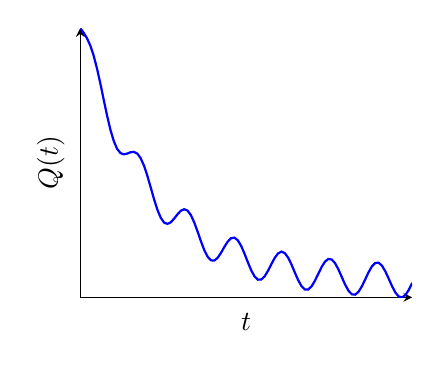
\begin{tikzpicture}
  \begin{axis}[ 
  	height=5cm,
    xlabel=$t$,
    ylabel={$Q(t)$},
    axis lines=left,
    xtick=\empty,
	ytick=\empty
  ] 
    \addplot[blue,samples=100,thick,domain=0:2*pi] {1.5*e^(-0.75*x)+0.1*sin(400*x)}; 
  \end{axis}
\end{tikzpicture}

\subsubsection{\(V(t) = \mathrm{square}(t)\)}
%\begin{tikzpicture}[domain=0:14]
%\draw (0,0) -- (0,4);
%\draw (0,4) -- (2,4);
%\draw (2,4) -- (2,0) node[anchor=west] {\(\pi\)};
%\draw (2,0) -- (2,-4) -- (4,-4) -- (4,4) -- (6,4) -- (6,-4);

%\draw[color=blue]
%plot (\x,{exp(-\x) + 0.35*sin(5*\x r)})
%node[right] {$f(x) = \sin x$};
%\end{tikzpicture}
\[
V(t)= \sum _{n = (1,3,5,\dots)} \frac{4}{n \pi} \sin (n t) =
\frac{4}{ \pi} \sin (n t) + \frac{4}{3 \pi} \sin (3 t) +
+ \frac{4}{5 \pi} \sin (5 t) \frac{4}{7 \pi} \sin (7 t) + \cdots
\]

Έτσι γίνεται η ανάλυση \textlatin{Fourier}, και αυτό θα το δούμε την επόμενη Τετάρτη, που θα πάμε στο Κεφάλαιο 8, που λέει σειρές \textlatin{Fourier}.

\[
V_N(t) = \sum _{n = (1,3,5,\dots)}^N \frac{4}{n \pi} \sin (n t)
\]
\[
V(t) = \sum _{n = (1,3,5,\dots)}^\infty \frac{4}{n \pi} \sin (n t) = \lim_{t \to \infty} V_N(t)
\]

\paragraph{}
Άρα:
\[
 \frac{\dif R}{\dif t}  + \frac{1}{RC}Q(t) = \frac{V_0 \sin (nt)}{R} \implies
 Q_n(t) = \frac{V_0C^2Rn}{C^2R^2n^2+1}e^{\frac{t}{RC}} + \frac{CV_0\sin (nt) - C^2RnV_0 \cos (nt)}{C^2R^2n^2+1}
\]

Οπότε αν:
\[
 \frac{\dif R}{\dif t}  + \frac{1}{RC}Q(t) = \frac{4}{\pi} \frac{\sin (nt)}{R} \implies
 Q_1(t) = \frac{4}{\pi} \left( \frac{C^2R}{C^2R^1+1} e^{-\frac{1}{RC}}+ \cdots \right)
\]
\[
 \frac{\dif R}{\dif t}  + \frac{1}{RC}Q(t) = \frac{4}{3\pi} \frac{\sin (3t)}{R} \implies
 Q_3(t) = \frac{4}{3\pi} \left( \frac{3C^2R}{9C^2R^1+1} e^{-\frac{1}{RC}}+ \cdots \right)
\]
\[
 \frac{\dif R}{\dif t}  + \frac{1}{RC}Q(t) = \frac{4}{5\pi} \frac{\sin (5t)}{R} \implies
 Q_5(t) = \cdots
\]

Άρα:
\[
Q(t) = \sum_{n \in \lbrace1,3,5,\dots\rbrace}Q_n(t)
\]

Γιατί όμως, αν \(V_1(t) \rightarrow Q_1(t), \ V_2(t) \rightarrow Q_2(t)\), τότε \(k_1V_1+k_2V_2 = k_1Q_1 +k_2Q_2\) σε αυτό το κύκλωμα (αρχή επαλληλίας/γραμμικότητα)?


\end{document}
